\documentclass[a4paper,11pt,landscape,twocolumn]{article}

\usepackage{../préambule}
\usepackage{clipboard}
\usetikzlibrary{arrows.meta,calc}

\makeatletter
\renewcommand{\maketitle}{%
{\scriptsize colle dans ton cahier d'exercices}
	\begin{center}
		\LARGE
		\myuline{\@title}
		\vspace{0.5em}
	\end{center}
}
\makeatother

\title{Activité : Chasse au trésor 2}
\date{}
\author{}

\begin{document}

\maketitle

Reproduit le repère ci-dessous sur ton cahier d'exercices :

\begin{center}
	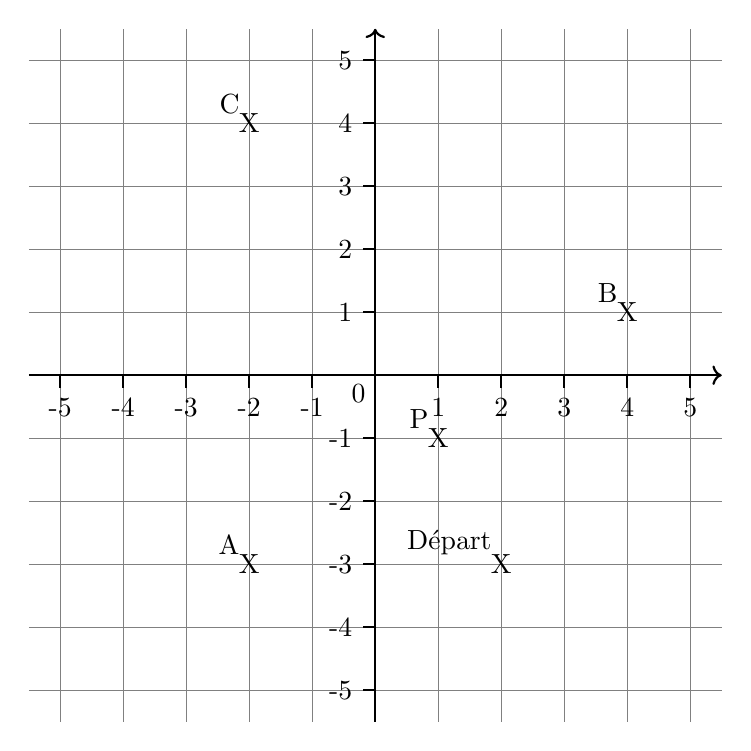
\begin{tikzpicture}[scale=0.8]
		\draw[ultra thin,gray] (-5.5,-5.5) grid (5.5,5.5);
		\draw[thick,->] (-5.5,0) -- (5.5,0);
		\draw[thick,->] (0,-5.5) -- (0,5.5);
		\foreach \x in {1,...,5} {
				\draw[thick] (\x,0) -- (\x,-0.2) node[below] {\x};
				\draw[thick] (-\x,0) -- (-\x,-0.2) node[below] {-\x};
				\draw[thick] (0,\x) -- (-0.2,\x) node[left] {\x};
				\draw[thick] (0,-\x) -- (-0.2,-\x) node[left] {-\x};
			}
		\node[below left] at (0,0) {0};

		\coordinate (Départ) at (2,-3);
		\coordinate (P) at (1,-1);
		\path let \p1 = (Départ) in coordinate (A) at (-\x1,\y1);
		\coordinate[rotate around={180:(P)}] (B) at (A);
		\coordinate (C) at ($(-6,3) + (B)$);

		\foreach \p in {Départ,A,P,B,C} {
				\node at (\p) {X};
				\node[above left] at (\p) {\p};
			}
	\end{tikzpicture}
\end{center}

Suit les instructions suivantes pour trouver le trésor :
\begin{enumerate}
	\item Commence au point \textbf{Départ} d'abscisse $2$ et d'ordonnée $-3$.
	\item Place le point \textbf{A} symétrique de Départ par rapport à \textbf{l'axe des ordonnées}.
	\item Place le point $P$ au coordonnées $(1;-1)$.
	\item Place le point \textbf{B}, symétrique de A par rapport à P.
	\item Pars du point B, et
	      \begin{itemize}
		      \item Monte de 3 graduations ;
		      \item Va vers la gauche de 6 graduations.
	      \end{itemize}
	      Place alors un point \textbf{C}.
\end{enumerate}



\end{document}